%%%%%%%%%%%%%%%%%%%%%%%%%%%%%%%%%%%%%%%%%%%%%%%%%%%%%%%%%%%%%%%%%%%%%%
% How to use writeLaTeX: 
%
% You edit the source code here on the left, and the preview on the
% right shows you the result within a few seconds.
%
% Bookmark this page and share the URL with your co-authors. They can
% edit at the same time!
%
% You can upload figures, bibliographies, custom classes and
% styles using the files menu.
%
%%%%%%%%%%%%%%%%%%%%%%%%%%%%%%%%%%%%%%%%%%%%%%%%%%%%%%%%%%%%%%%%%%%%%%

\documentclass[12pt]{article}

\usepackage{sbc-template}

\usepackage{graphicx,url}

% \usepackage[brazil]{babel}   
\usepackage[utf8]{inputenc}  

     
\sloppy

\title{Instruções para Autores de Artigos e Resumos\\ de Conferências da SBC}

\author{Luciana P. Nedel\inst{1}, Rafael H. Bordini\inst{2}, Flávio Rech
  Wagner\inst{1}, Jomi F. Hübner\inst{3} }


\address{Instituto de Informática -- Universidade Federal do Rio Grande do Sul
  (UFRGS)\\
  Caixa Postal 15.064 -- 91.501-970 -- Porto Alegre -- RS -- Brazil
\nextinstitute
  Departamento de Ciência da Computação -- Universidade de Durham\\
  Durham, Reino Unido
\nextinstitute
  Departamento de Sistemas e Computação\\
  Universidade Regional de Blumenal (FURB) -- Blumenau, SC -- Brazil
  \email{\{nedel,flavio\}@inf.ufrgs.br, R.Bordini@durham.ac.uk,
  jomi@inf.furb.br}
}

\begin{document} 

\maketitle

\begin{resumo} 
  Este meta-artigo descreve o estilo a ser usado na confecção de artigos e
  resumos de artigos para publicação nos anais das conferências organizadas
  pela SBC. É solicitada a escrita de resumo e abstract apenas para os artigos
  escritos em português. Artigos em inglês deverão apresentar apenas abstract.
  Nos dois casos, o autor deve tomar cuidado para que o resumo (e o abstract)
  não ultrapassem 10 linhas cada, sendo que ambos devem estar na primeira
  página do artigo.
\end{resumo}

     

\begin{abstract}
  Este meta-artigo descreve o estilo a ser usado em artigos e artigos curtos
  para as conferências da SBC. Para artigos em inglês, você deve adicionar apenas um
  abstract, enquanto para os artigos em português, também pedimos um resumo em
  português (``resumo''). Em ambos os casos, os resumos não devem ter mais de
  10 linhas e devem estar na primeira página do artigo.
\end{abstract}


\section{Informações Gerais}

Todos os artigos completos e pôsteres (artigos curtos) submetidos a alguma conferência da SBC,
incluindo quaisquer documentos de apoio, devem ser escritos em inglês ou em
português. O formato do papel deve ser A4 com coluna única, margem superior de 3,5 cm, 
margem inferior de 2,5 cm e margens laterais de 3,0 cm, sem
cabeçalhos ou rodapés. A fonte principal deve ser Times, tamanho nominal de 12
pontos, com 6 pontos de espaço antes de cada parágrafo. Os números das páginas
devem ser suprimidos.

Os artigos completos devem respeitar os limites de página definidos pela conferência.
Conferências que publicam apenas resumos pedem por textos de \textbf{uma} página.

\section{Primeira Página} \label{sec:firstpage}

A primeira página deve exibir o título do artigo, o nome e o endereço dos
autores, o abstract em inglês e o resumo em português (resumos são
necessários apenas para artigos escritos em português). O título deve ser centralizado
em toda a página, em fonte negrito de 16 pontos e com 12 pontos de espaço
antes de si. Os nomes dos autores devem ser centralizados em fonte de 12 pontos, negrito, todos
dispostos na mesma linha, separados por vírgulas e com 12 pontos de
espaço após o título. Os endereços devem ser centralizados em fonte de 12 pontos, também com
12 pontos de espaço após os nomes dos autores. Os endereços de e-mail devem ser
escritos usando a fonte Courier New, tamanho nominal de 10 pontos, com 6 pontos de espaço
antes e 6 pontos de espaço depois. O abstract e o resumo (se for o caso) devem estar em fonte Times de 12 pontos,
com recuo de 0,8 cm em ambos os lados. A palavra \textbf{Abstract} e \textbf{Resumo},
deve ser escrita em negrito e preceder o texto.

\section{CD-ROMs e Anais Impressos}

Em algumas conferências, os artigos são publicados em CD-ROM enquanto apenas o
resumo é publicado nos Anais impressos. Neste caso, os autores são
convidados a preparar duas versões finais do artigo. Uma, completa, para ser
publicada no CD e a outra, contendo apenas a primeira página, com
abstract e resumo (para artigos em português).

\section{Seções e Parágrafos}

Os títulos das seções devem estar em negrito, 13pt, alinhados à esquerda. Deve haver um espaço extra
de 12 pt antes de cada título. A numeração das seções é opcional. O primeiro
parágrafo de cada seção não deve ser recuado, enquanto as primeiras linhas dos
parágrafos subsequentes devem ser recuadas em 1,27 cm.

\subsection{Subseções}

Os títulos das subseções devem estar em negrito, 12pt, alinhados à esquerda.

\section{Figuras e Legendas}\label{sec:figs}


As legendas de figuras e tabelas devem ser centralizadas se tiverem menos de uma linha
(Figura~\ref{fig:exampleFig1}), caso contrário, justificadas e recuadas em 0,8 cm em
ambas as margens, como mostrado na Figura~\ref{fig:exampleFig2}. A fonte da legenda deve
ser Helvetica, 10 pontos, negrito, com 6 pontos de espaço antes e depois de cada
legenda.

\begin{figure}[ht]
\centering
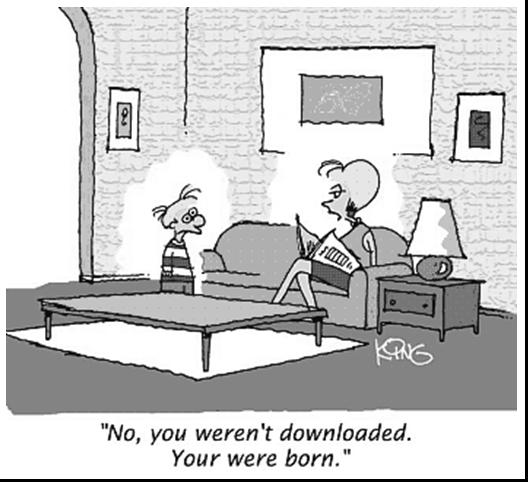
\includegraphics[width=.5\textwidth]{fig1.jpg}
\caption{Uma figura típica}
\label{fig:exampleFig1}
\end{figure}

\begin{figure}[ht]
\centering
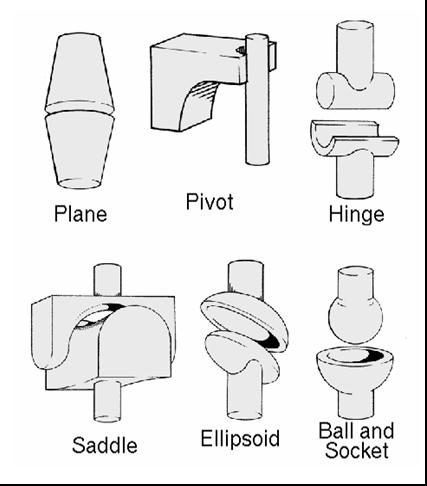
\includegraphics[width=.3\textwidth]{fig2.jpg}
\caption{Esta figura é um exemplo de uma legenda de figura que ocupa mais de uma
linha e é justificada considerando as margens mencionadas na Seção~\ref{sec:figs}.}
\label{fig:exampleFig2}
\end{figure}

Em tabelas, tente evitar o uso de fundos coloridos ou sombreados, e evite
linhas de enquadramento grossas, duplas ou desnecessárias. Ao relatar dados empíricos,
não use mais dígitos decimais do que o justificado por sua precisão e
reprodutibilidade. A legenda da tabela deve ser colocada antes da tabela (ver Tabela 1)
e a fonte usada também deve ser Helvetica, 10 pontos, negrito, com 6 pontos de
espaço antes e depois de cada legenda.

\begin{table}[ht]
\centering
\caption{Variáveis a serem consideradas na avaliação de técnicas de
interação}
\label{tab:exTable1}
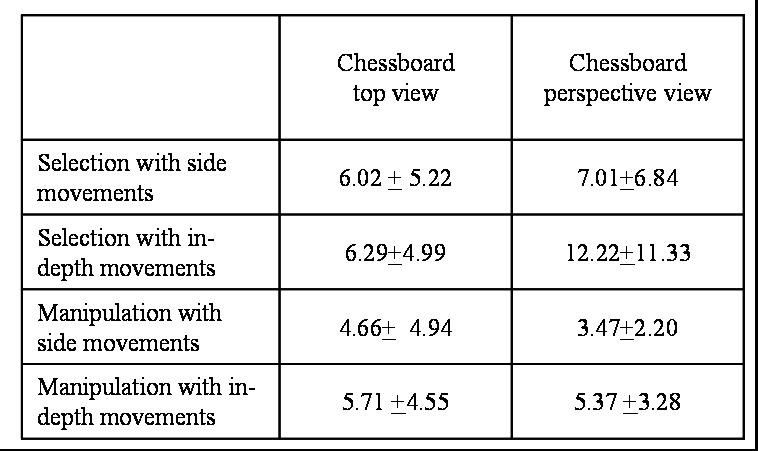
\includegraphics[width=.7\textwidth]{table.jpg}
\end{table}

\section{Imagens}

Todas as imagens e ilustrações devem ser em preto e branco, ou tons de cinza,
exceto para os artigos que estarão disponíveis eletronicamente (em CD-ROMs,
internet, etc.). A resolução da imagem no papel deve ser de cerca de 600 dpi para
imagens em preto e branco, e 150-300 dpi para imagens em tons de cinza. Não inclua
imagens com resolução excessiva, pois elas podem levar horas para imprimir, sem qualquer
diferença visível no resultado.

\section{Referências}

As referências bibliográficas devem ser inequívocas e uniformes. Recomendamos fornecer
as referências dos nomes dos autores entre colchetes, por exemplo, \cite{knuth:84},
\cite{boulic:91}, e \cite{smith:99}. As referências devem ser listadas usando fonte de tamanho 12, com 6 pontos de espaço
antes de cada referência. A primeira linha de cada referência não deve ser
recuada, enquanto as subsequentes devem ser recuadas em 0,5 cm.

\bibliographystyle{sbc}
\bibliography{sbc-template.bib}

\end{document}
